\pagenumbering{arabic}
\chapter{Einleitung}
\label{c:intro}

Inhalt dieser wissenschaftlichen Arbeit ist das automatische Erstellen einer Material-Kostengliederung aus einer \ac{ifc}-Datei mithilfe von \ac{nlp} zur Erweiterung einer Bausoftware. Diese Bausoftware ist die ORCA AVA aus dem mittelständigen Softwarehaus \glqq ORCA Software GmbH\grqq{} aus Neubeuern. 
In diesem Kapitel soll eine kurze Einführung über die \glqq ORCA Software GmbH\grqq{} und das Produkt  ORCA AVA gegeben werden. Außerdem wird die Motivation für die Programmerweiterung und die wissenschaftliche Vorgehensweise dieser Arbeit beschrieben.

\section{Ausgangssituation}
\label{c:intro:start}

Die im Titel beschriebene Bausoftware ist die ORCA AVA aus dem Softwarehaus \glqq ORCA Software GmbH\grqq{}. Dieses wurde im Jahr 1990 von Dipl.-Ing. Siegfried Tille und Dipl.-Ing. Heinz Nießen gegründet. Der Hauptsitz des Unternehmens ist in Neubeuern, bei Rosenheim. Das Unternehmen ist auf die Produktentwicklung von Software für die Baubranche spezialisiert. Im Vordergrund stehen die Ausschreibungssoftware ORCA AVA und die Ausschreibungstext-Plattform \ac{ade}. Ziel der Entwicklung ist es die \ac{ava} eines Bauvorhabens für Planer, Architekten und Bauingenieure zu vereinfachen. Der Leitfaden ist, Software zu entwickeln, die jeder versteht, intuitiv bedienbar ist, einen optimalen Workflow gewährleistet und viele Import- und Exportmöglichkeiten für den Datenaustausch bietet.
Diese Arbeit fokussiert sich auf eine Erweiterung der ORCA AVA. Sie ist für alle Architektur- und
Ingenieurbüros, Wohnungsbaugesellschaften, Unternehmen und Behörden zur einfachen Abwicklung von Bauprojekten mit Ausschreibung, Vergabe und Abrechnung. Zusätzlich bildet sie das Kostenmanagement von solchen Projekten ab. Die Software ist außerdem \ac{bim} fähig und bietet \ac{din} zertifizierte Schnittstellen für den Datenaustausch an. Neben der ORCA AVA gibt es den \ac{ifc}-Manager als eigene Instanz, der \ac{ifc}-Modelle anzeigen kann. Die ORCA AVA kann dann Mengen aus dem Gebäudemodell übernehmen.
Es stehen drei verschiedene Editionen der Software zur Verfügung. Die ORCA AVA \ac{se}, die ORCA AVA \ac{pe} und die ORCA AVA \ac{ee}. Die aktuellste Version ist die 25.0.

Technisch wird die ORCA AVA in .NET entwickelt. Ein Großteil der Anwendung besteht noch aus \ac{vb} Code. Alle neuen Komponenten und Erweiterungen werden in C\# implementiert. Neue \ac{gui}-Komponenten werden dementsprechend mit \ac{wpf} entwickelt. \ac{wpf} ist ein .NET Framework für das Erstellen von Windows Applikationen mit grafischer Benutzeroberfläche von Microsoft. \citep{Microsoft_2022} Die ORCA AVA und der \ac{ifc} Manager (siehe Abschnitt \ref{c:basics:ifc:usage}) laufen in eigenen Prozessen und kommunizieren auf Prozessebene in der lokalen Umgebung. 

\section{Motivation}
\label{c:intro:motivation}

Ziel der \glqq ORCA Software GmbH\grqq{} ist es, \ac{bim} noch mehr in die ORCA AVA zu integrieren. \ac{bim} bedeutet, dass die Planung von Bauprojekten vollständig auf digitaler Basis durchgeführt wird.  Für jeden Projektbeteiligten besteht somit jederzeit Zugriff auf alle projektrelevanten Daten über Kosten, Mengen und Zeitabläufen. Somit können Baukosten einfacher ermittelt und der Bauprozess besser überwacht werden. In Abbildung \ref{fig:bim} ist zu sehen, dass \ac{bim} ein relevanter Begriff in der Baubranche ist. Die Verwendung der Praxis ist allerdings noch nicht verbreitet. \citep[p.~20]{Thomas_Baumanns_Dr_Philipp-Stephan_Freber_Dr_Kai-Stefan_Schober_Dr_Florian_Kirchner2016-gu} Mit dem \glqq \ac{ifc} First\grqq{} Ansatz ist das langfristige Ziel der ORCA AVA das Thema \ac{bim} noch mehr abzudecken. Aus den Daten eines 3D-Gebäudemodells soll automatisch ein Ausschreibungstext erstellt werden können. Bauteile aus dem Gebäudemodell sollen dann mit Kurztext, Langtext, Menge, Preis und vordefinierten Kostengliederungen in den Programmteil Bauelemente der ORCA AVA übernommen werden. Aufgrund der hohen Relevanz des Themas, spricht das Ganze viele Kunden an und stellt somit ein effektives Werbemittel für den Verkauf der Software dar. Ein Teil des langfristigen Ziels ist die Übernahme der Baumaterialien aus einer \ac{ifc}-Datei. Diese bietet die erste Kostengliederung für den \glqq \ac{ifc} First\grqq{} Ansatz. Die Übernahme von weiteren Daten aus dem \ac{ifc}-Modell können darauf aufgebaut werden.

\begin{figure}[h]
	\centering
	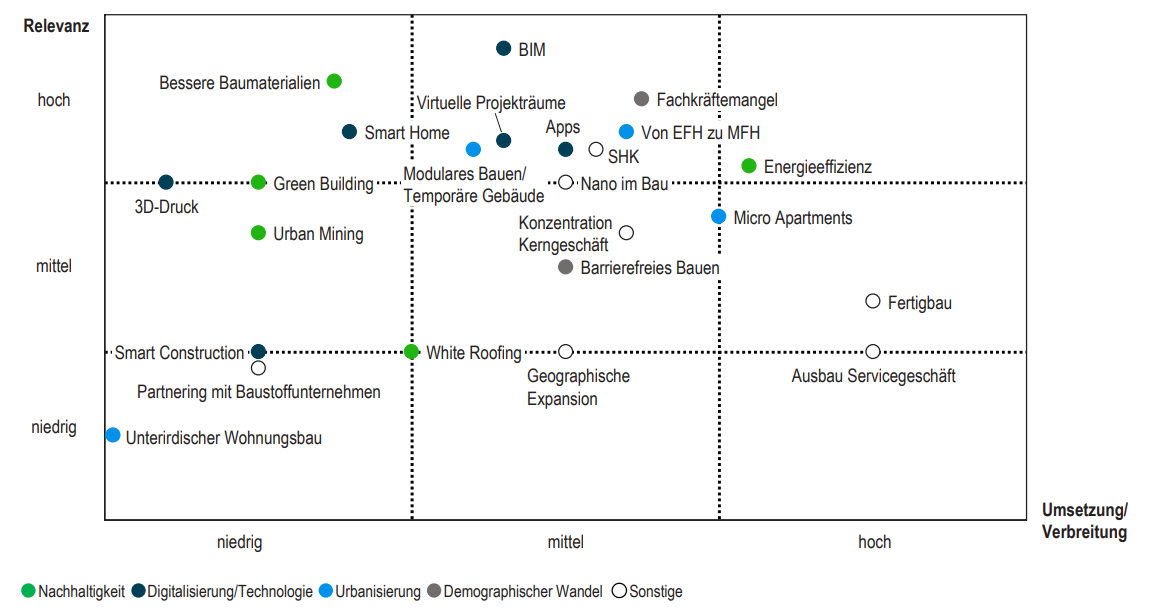
\includegraphics[scale=0.52]{bim-relevanz}
	\caption[Relevanz \ac{bim}]
	{Megatrends Nachhaltigkeit und Digitalisierung in der Bauwirtschaft. Bilder aus \citep[p.~20]{Thomas_Baumanns_Dr_Philipp-Stephan_Freber_Dr_Kai-Stefan_Schober_Dr_Florian_Kirchner2016-gu}}
	\label{fig:bim}
\end{figure}
Ein weiterer Trendbegriff, der mit der Programmerweiterung abgedeckt werden soll, ist \glqq Künstliche Intelligenz\grqq{} und \glqq Maschinelles Lernen\grqq{}. Das Suchinteresse der beiden Themen ist in Abbildung \ref{fig:ki-ml-trend} zu sehen. Die Werte geben das Google-Suchinteresse relativ zum höchsten Punkt im angegebenen Zeitraum an. Der Begriff \glqq Maschinelles Lernen\grqq{} hat seit Anfang 2015 ein steigendes Suchinteresse. Bei \glqq Künstliche Intelligenz\grqq{} ist das Suchinteresse von Anfang 2017 bis Ende 2021 konstant hoch. Der starke Anstieg ab November 2022 ist signifikant und korreliert mit der Veröffentlichung der Software ChatGPT. Man erkennt insgesamt, dass das Interesse über die letzten Jahre stetig ansteigt. Die Abdeckung dieser Begriffe ist seit geraumer Zeit ein Wunsch der Vertriebsseite für den noch besseren Verkauf der Software. Die Erweiterung wäre der erste Einsatz von maschinellem Lernen. Es ist also zusätzlich auch ein Pilotprojekt in der ORCA AVA Entwicklung, um sich mit Machine-Learning-Algorithmen vertraut zu machen und Erfahrungen in diesem Themengebiet zu bekommen.

Durch die genannten Punkte ist die Programmerweiterung dem Kano-Modell nach als Begeisterungsfeature zuzuordnen. Die Kundenzufriedenheit steigt also exponentiell mit dem Erfüllungsgrad der Anforderung. (siehe Abbildung \ref{fig:kano-model}) Mit der Zeit wandelt sich es dann erst in ein Leistungsfeature und irgendwann in ein Basisfeature. \citep[p.~3-4]{Hölzing_2008} Es besteht also die Motivation die Erweiterung möglichst exklusiv zur Verfügung zu stellen. Es eignet sich somit sehr für die ORCA AVA \ac{ee} Edition.

\begin{figure}[tb]
	\centering
	
	\begin{subfigure}{0.99\textwidth}
		\centering
	\includegraphics[width=1\textwidth]{künstiliche-intilligenz-trend}
		\caption{Suchinteresse: Künstliche Intelligenz}
		\label{FIG:ki-trend}
	\end{subfigure}
	\hspace{1cm}
	\begin{subfigure}{0.99\textwidth}
		\centering
	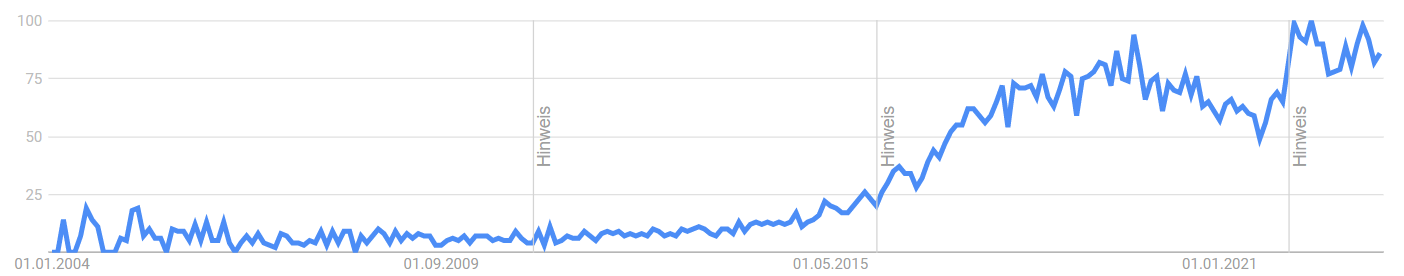
\includegraphics[width=1\textwidth]{machine-learning-trend}
		\caption{Suchinteresse: Machine Learning}
		\label{FIG:ml-trend}
	\end{subfigure}
	
	\caption[Google Trends]{Google Suchinteresse der beiden Begriffe \glqq Künstliche Intelligenz\grqq{} und \glqq Maschinelles Lernen{} seit 2004 bis 2023}
	\label{fig:ki-ml-trend}
\end{figure}

\begin{figure}[h]
	\centering
	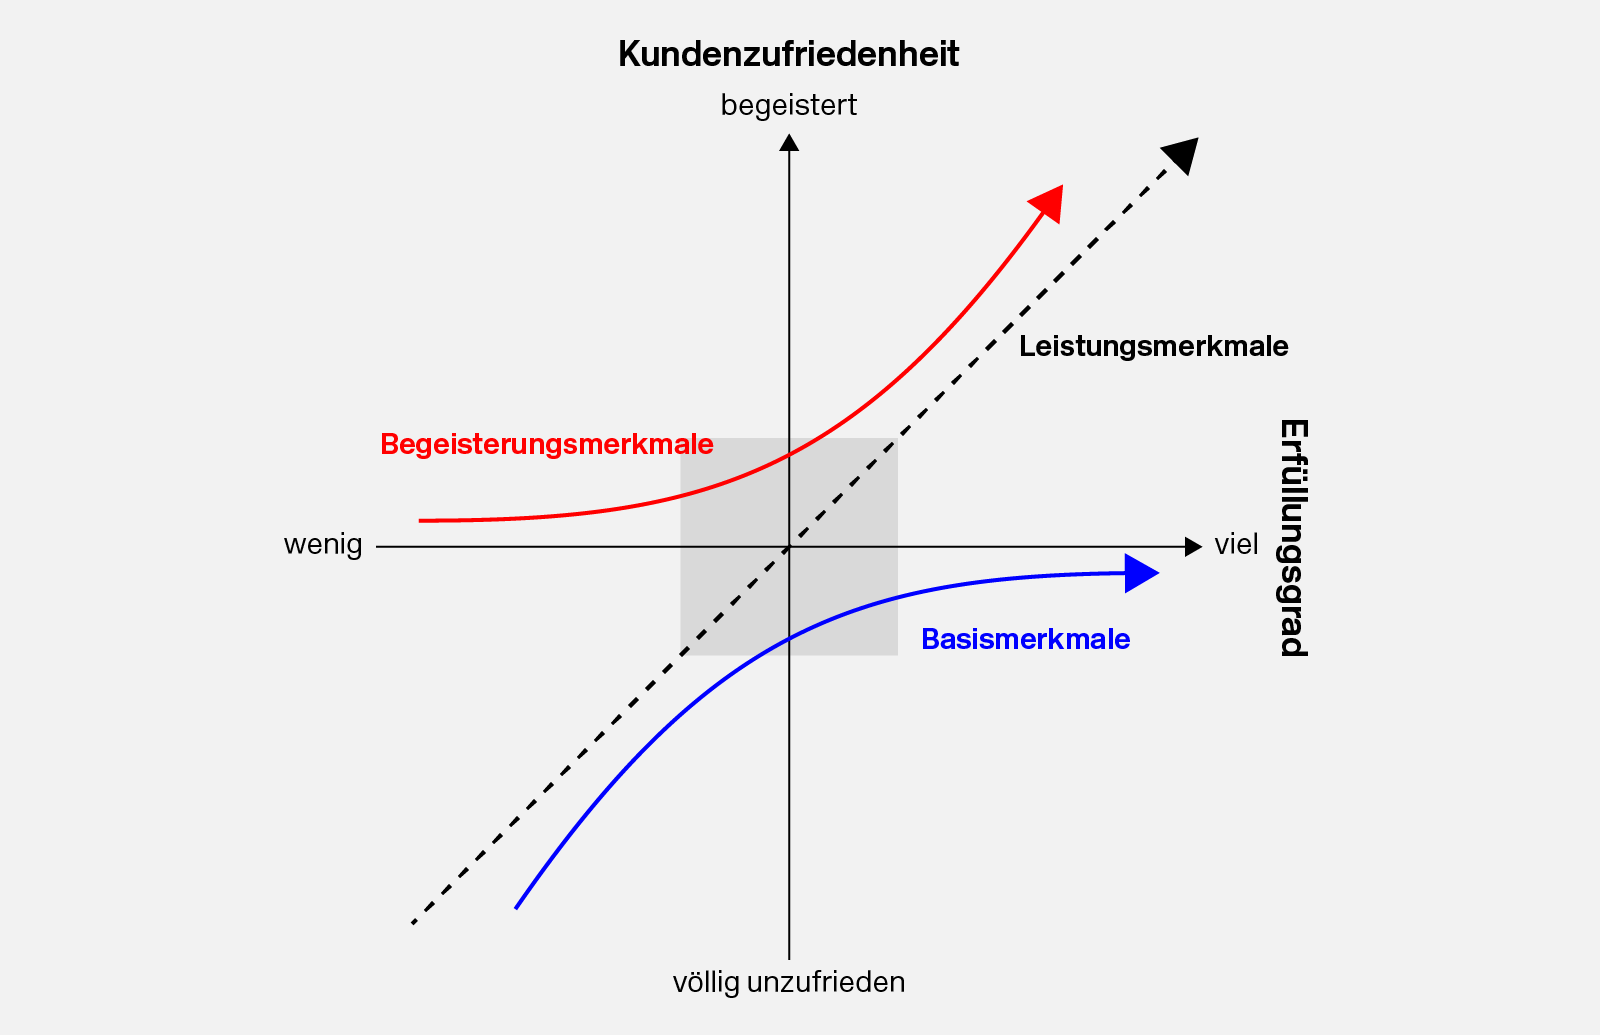
\includegraphics[width=\textwidth]{kano-modell}
	\quelle{https://dmexco-lightsails-media.s3.eu-central-1.amazonaws.com/wp-content/uploads/2021/01/04112832/Kano-Modell.png (Accessed: 2023-2-24) }
	\caption[Kano Modells]{Kano Modell der Kundenzufriedenheit}
	\label{fig:kano-model}
\end{figure}

\section{Ziel der Arbeit}
\label{c:intro:target}
Um die Anforderungen aus Abschnitt \ref{c:requirements:requirements} umsetzten zu können, muss zuvor ein Ziel formuliert werden.
Die Zieldefinition für diese Arbeit wird nach der SMART Technik definiert. Dabei muss ein Ziel folgende Eigenschaften haben:

\begin{itemize}
	\setlength\itemsep{0.01em}
	\item Spezifisch
	\item Messbar
	\item Attraktiv
	\item Realisierbar
	\item Terminiert
\end{itemize}

Anhand dieser Kriterien wurde folgendes Ziel definiert:


\goalshaded{Bis zum 15.06.2023 wird eine \glqq Draftprojekt\grqq{} mit allen vollständigen funktionalen Anforderungen für die ORCA AVA implementiert. Für die Implementierung werden passende Algorithmen nach den Kriterien der Messbarkeit (siehe Abschnitt \ref{c:requirements:requirements:functional}) ausgewählt. Zusätzlich sollen die Maßnahmen zur Qualitätssicherung (Kapitel \ref{c:qs}) durchgeführt werden und die Qualitätssicherungs-Abteilung alle Funktionen freigegeben haben.}

\section{Wissenschaftliche Vorgehensweise}
\label{c:intro:methodology:scientific_proceture}
Im Folgenden wird die wissenschaftliche Vorgehensweise der Arbeit aufgezeigt.
In Abschnitt\,\ref{c:intro} wurde bereits die Ausgangssituation beschrieben, das Entwickeln der Programmerweiterung motiviert und des Ziel dieser Arbeit definiert. Im nächsten Kapitel, Kapitel\,\ref{c:basics}, werden Grundlagen erläutert, auf die diese Arbeit aufbaut. Im anschließenden Kapitel\,\ref{c:requirements} sollen die Problemstellung und Anforderungen analysiert werden. Danach (Kaptiel\,\ref{c:theoretical}) wird eine Lösung für die Problemstellung theoretisch konzipiert und verschiedene mögliche Algorithmen analysiert. In Kapitel\,\ref{c:comparison} werden die Algorithmen gegenübergestellt und nach den definierten Kriterien ausgewählt. Kapitel\,\ref{c:qs} zeigt die genutzten Maßnahmen der Qualitätssicherung auf. Am Ende wird das Ergebnis bewertet und ein Ausblick gegeben.
\todo{Muss noch vervollständigt werden}

\chapter{Grundlagen}
\label{c:basics}
In diesem Kapitel werden die Grundlagen im Bereich der fachspezifischen Themen, Technik und Projektmanagement vermittelt. Das soll Verständnis für die folgenden Kapitel schaffen. Zuerst geht es um das Projektmanagement. Anschließend geht es um das Format \ac{ifc}, dessen Geschichte und dessen Nutzungsmöglichkeiten für diese Arbeit. Außerdem wird die Struktur und der Nutzen einer Kostengliederung in der ORCA AVA veranschaulicht.

\section{Projektmanagement}
\label{c:basics:project-management}
Bevor auf technische und fachliche Aspekte von \ac{ifc} und Kostengliederungen eingegangen wird, folgt die Einführung in das Projektmanagements mit SCRUM und \ac{devops}.

\subsection{Vorgehensmodell}
\label{c:basics:project-management:procedure_model}
Das Projekt wurde mithilfe agiler Softwareentwicklung durchgeführt. Im ORCA AVA Entwicklungsteam wird das SCRUM Modell verwendet. Die Entwicklung der Produkterweiterung in dieser Arbeit läuft in diesem SCRUM-Prozess.

\begin{definition}[Scrum]
	\glqq Scrum is a lightweight framework that helps people, teams and organizations generate value through adaptive solutions for complex problems. \grqq{} \citep[p.~3]{scrum_2020}
\end{definition}

SCRUM verwendet einen iterativen, inkrementellen Ansatz. So kann Sprint für Sprint aus gewonnenen Erfahrungen der Entwicklungsablauf optimiert werden. \citep{scrum_2020} Product Owner in der ORCA AVA Entwicklung ist die \glqq ORCA Software GmbH\grqq{}, in Vertretung des Produktmanagement-Teams. Die Umsetzung der Sprint-Ziele wird von einer Person implementiert.

\subsection{DevOps}
\label{c:basics:project-management:devops}
Die Bezeichnung \ac{devops} vereint die beiden Praktiken \glqq Development\grqq{}(Entwicklung) und \glqq Operations\grqq{}(Vorgänge). Die traditionelle Trennung von Entwicklung und Softwarebetrieb führt oft zu
Interessenskonflikten. Entwickler wollen stetig die Software verbessern und der Betrieb will Änderungen vermeiden, um die Stabilität des Systems zu gewährleisten. Durch \ac{devops} entsteht ein Softwareentwicklungsprozess, den man durch Praktiken wie Continous Integration, Continous Delivery, Continous Deployment, automatisiertes Teste, Infrastructure-as-Code und automatische Veröffentlichungen beschleunigt. DevOps steht auch für eine Entwicklungskultur mit offener Zusammenarbeit, Kommunikation, Transparenz und Eingestehen von Fehlern, um Konflikte im Team zu vermeiden. \citep{devops_2021} Im Entwicklungsteam der ORCA AVA wird diese Praktik umgesetzt. Die technischen Hilfsmittel, die für den DevOps Prozess verwendet werden, sind in Abschnitt \ref{c:qs:technical_aids} beschrieben.

\section{\ac{ifc}}
\label{c:basics:ifc}
Die Daten für die Material-Kostengliederung werden aus einem digitalem Gebäudemodell entnommen. Der öffentliche internationale Standard (ISO 16739-1:2018) für Gebäudemodelle ist \ac{ifc}. \citep{BuildingSMART_IFC4_doc} Dieser wird auch in der bestehenden ORCA AVA benutzt, um den Ausschreibungsprozess zu unterstützen. \ac{ifc} Dateien können geöffnet, angeschaut und Informationen über das Modell in die Hauptsoftware übernommen werden. Im folgenden Kapitel wird die Geschichte, das Format von \ac{ifc} und die Verwendung in der ORCA AVA erläutert.

\subsection{Geschichte}
\label{c:basics:ifc:history}
\ac{ifc} ist die Hauptleistung der buildingSMART International, Ltd.  Die non-profit Organisation will mit der Spezifikation den BIM Prozess fördern und voranbringen. \citep{BuildingSMART_IFC}
Angefangen hat die Organisation als der Verein \textit{Industrieallianz für Interoperabilität IAI e. V.} mit Sitz in Berlin. 1994 startete die Entwicklung an dem offenen Datenmodellstandard \ac{ifc}. Dieser sollte die Anforderungen der Industrie an Interoperabilität gerecht werden und eine gemeinsame Basis zum Austausch von Informationen durch verschiedenen Anwendungen schaffen. Im Zusammenhang mit \ac{bim} sollten Daten lesbar, editierbar für verschiedene Systeme durch den Bauprozess und kompletten Lebenszyklus eines Gebäudes geteilt werden. \citep{Laakso2012-oi} Nach einigen Prototypen wurde 1999 \ac{ifc} 2.0 veröffentlicht. Diese wurde bis 2007 mit der Version 2.3.0.1 stetig verbessert. Die Version 2.3 wird auch in heutigen Projekten noch verwendet. 2013 wurde \ac{ifc}4 veröffentlicht, welche mit der Version 4.0.2.1 die aktuellste, offizielle \ac{ifc} Version ist. Das Format wird weiterhin stetig weiterentwickelt. Neue Versionen stehen schon vor einer Abstimmung der \ac{iso}. \citep{BuildingSMART_history_2022} Es gibt folgendermaßen aktuell zwei offizielle Versionen. Beide werden in der Praxis benutzt und sind, wie in Abschnitt \ref{c:basics:ifc:usage} beschrieben, mit der ORCA AVA kompatibel.


\subsection{Format}
\label{c:basics:ifc:format}
Das \ac{ifc} Format kodiert folgende Daten:
\begin{itemize}
	\item Identität, Semantik, Attribute und Relationen von Objekten
	\item Abstrakte Konzepte wie Performance oder Kosten
	\item Prozesse wie z.B.Installationen und Operationen
	\item Personen wie z.B. Eigentümer oder Lieferanten
\end{itemize}
Die Spezifikation kann also für das Bauen, Betreiben oder Nutzen eines Gebäudes genutzt werden. \ac{ifc} ist ein Implementierungs-Unabhängiges Datenmodell, welches in verschiedenen Umgebungen und elektronischen Formaten benutzt werden kann. Es kann beispielsweise in eine relationales Datenbankschema gegossen oder auch als Dateiformat implementiert werden. Das weitverbreiteste Format ist \ac{spf} \citep{Laakso2012-oi,BuildingSMART_IFC}. \ac{spf} ist das kompakteste Format für den dateibasierten Import und Export von \ac{ifc}-Dateien. Die Dateiendung des Formates ist \glqq \textit{.ifc}\grqq{}. Des Weiteren kann \ac{ifc} als \ac{xml} oder ZIP Datei verwendet werden. \citep{BuildingSMART_IFC}

\subsection{Verwendung}
\label{c:basics:ifc:usage}
\begin{displayquote}
	\glqq Today, \ac{ifc} is typically used to exchange information from one party to another for a specific business transaction.\grqq{} \citep{BuildingSMART_IFC}
\end{displayquote}
In der ORCA AVA wird \ac{ifc} für das Einlesen und Übernehmen von Maßen und Mengen in die Ausschreibung verwendet. Es vereinfacht den Prozess, die in der \ac{cad}-Software erstellten Daten einfach in die Leistungsverzeichnisse der ORCA AVA zu überführen.
Die ORCA AVA kann \ac{ifc}-Dateien einlesen. Im \ac{ifc} Manager wird das 3D-Modell dann angezeigt. In dem geöffneten Fenster gibt es einige fachliche Ansichten, die jegliche \ac{ifc}-Daten nochmal fachlich abstrahieren. In den Ansichten können zum Beispiel bestimmte Maße oder die Anzahl verschiedener Bauteile, die aus dem \ac{ifc}-Modell berechnet werden, in die ORCA AVA übernommen werden. Auch alle im \ac{ifc} definierten Eigenschaften eines Bauteils sind in der Eigenschaften-Ansicht sichtbar. Hier kann man auch die Materialbezeichnung des Bauteils finden, die im Modell hinterlegt ist. In Abbildung\,\ref{fig:ifc-manager} ist die Oberfläche des \ac{ifc} Managers zu sehen. Man sieht die Materialangabe rechts unten im Eigenschaftenfeld unter dem 3D-Modell.

Für das Arbeiten mit \ac{ifc}-Dateien wird die open-source Bibliothek \textit{xbim-toolkit} verwendet. Die .NET Bibliothek kann \ac{ifc}-Dateien lesen, schreiben und anzeigen. Außerdem unterstützt es bei der Berechnung von komplexer Geometrie, um die Modelldaten für Analysen nutzbar zu machen. Die Entwicklung der Bibliothek startete 2007 und läuft seit 2009 in Zusammenarbeit mit der Norhumbria Untiversity. Mittlerweile bildet es die Standards \ac{ifc2x3} und \ac{ifc4} zu 100\% ab. Zudem bietet es an, auch \ac{ifc2x3} Modelle über das \ac{ifc4} Interface anzuprogrammieren. Somit können mit einer Codebasis beide Formate abgebildet und unterstützt werden. \citep{Xbim_ltd_history}


\subsection{Möglichkeiten für die  Materialangabe eines Bauteils}
\label{c:basics:ifc:buildingmaterial}
In einem \ac{ifc}-Modell können Materialien auf unterschiedliche Weise einem Bauteil zugewiesen werden. Die Spezifikation bietet die Klasse \textit{IfcMaterial}. Diese bildet fachlich ein Material ab. Es hat die Attribute Name, Description und Category.\citep{ifc_material} Eine Instanz von \textit{IfcMaterial} kann mit einem Element oder Elementtyp über die \textit{IfcRelAssociatesMaterial} verbunden werden. Diese Zuweisung kann über verschiedene Weisen stattfinden. In Abbildung \ref{fig:material-single} ist eine direkte Zuweisung über das \textit{IfcRefAssociatesMaterial} zu sehen. Hier hängt das \textit{IfcMaterial} direkt am Element. 
Bei einer Platte mit mehreren Schichten kann das \textit{IfcMaterial} auch wie in Abbildung \ref{fig:layer-set} zu sehen an einem \textit{IfcMaterialLayerSet} zugewiesen sein. Jede Schicht hat hier seine eigene Dicke und eigene Materialangabe. 
Ein Träger kann das \textit{IfcMaterial} über ein \textit{IfcMaterialProfileSet} abgebildet haben. (siehe Abbildung \ref{fig:profile-set})
Bei zum Beispiel einer Tür können verschiedene Materialien des Rahmens und der Verglasung über das \textit{IfcMaterialConstituentSet} abgebildet werden. (siehe Abbildung \ref{fig:constituent-set}) \citep{ifc_material_association}
Zusätzlich gibt es noch ältere Möglichkeiten Materialangaben an ein Element zu binden. In \ac{ifc2x3} gibt es die Klasse \textit{IfcMaterialList} \citep{Thomas2007_MaterialList}. Diese Möglichkeit ist deprecated, in der Praxis kommt das \ac{ifc2x3} Format noch regelmäßig vor. Die \textit{IfcMateGitOpsrialList} muss also auch beachtet werden.

Neben verschiedenen Verbindungen zu \textit{IfcMaterial} hat jedes Element bei \ac{ifc} auch verschiedene Property Sets. Property Sets sind Container, die Eigentschaften je nach ihrem Namensattribut enthalten. Einige Property Sets sind in der Spezifikation des \ac{ifc} Standards enthalten. Es können auch zusätzlich benutzerdefinierte Property Sets erfasst werden. Diese können auch Informationen über das Material eines Elements enthalten. \citep{ifc_property_set} Das PropertySet \textit{Pset\_MaterialConcrete} weist darauf hin, dass es sich z.B um Beton handelt.

\begin{figure}[h]
	\centering
	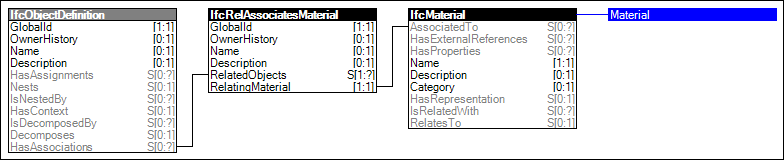
\includegraphics[width=\textwidth]{material-single}
	\caption[IfcMaterial]{Material Single Association}
	\label{fig:material-single}
\end{figure}

\section{Das Format Kostengliederung in der ORCA AVA}
\label{c:basics:coststructure}
Die Kostengliederung bietet eine Struktur, um Gesamtkosten einer Baumaßnahme in Kostengruppen unterteilt auswerten zu können. Logisch zusammengehörende Kosten können so in eine \ac{kg} zusammengerechnet werden. Außerdem handelt es sich beim Aufbau um eine Baumstruktur, wodurch Kostengruppen hierarchisch addiert werden können. In Abbildung \ref{fig:cost-structure} ist ein Beispiel einer Kostengliederung mit Materialien zu sehen. Der Gliederungspunkt \textit{Mineralisch} wird in die Unterpunkte \textit{Mauerwerk}, \textit{Beton}, \textit{Dachziegel} und \textit{Kies} unterteilt. Die Kosten der Unterpunkte können also für den Gliederungspunkt \textit{Mineralisch} addiert werden, um die Kosten aller Mineralien zu erfassen.
Bei einem Bauprojekt kann man so Kosten über alle Projektphasen vergleichen. Von der Kostenschätzung über die  Ausschreibung bis zur Rechnungsfreigabe. So können Kostenauswertungen nach den verschiedenen Kostengruppen durchgeführt werden. In einem ORCA AVA Projekt kann man verschiedene Kostengliederungen definieren. Es existieren bereits Standardkostengliederungen beim Erstellen eines neuen Projektes. Zusätzlich können neue Kostengliederungen erstellt oder importiert werden.\citep{helpdesk-kostengliederungen}


Technisch ist eine Kostengliederung als Modell im C\# Code definiert. Der Aufbau bildet die Baumstruktur über eine Referenz zur ParentNode und mehreren ChildrenNodes ab. Das Model kann über die ORCA AVA interne Middleware in der Datenbank persistiert werden. Die persistierten Kostengliederungen werden dann in entsprechenden Programmteilen angezeigt.
So müssen nach der generierten Kostengliederungs-Struktur die strukturierten Materialbezeichnungen in das C\# Modell abgebildet werden. So wird nach dem Import die erstellte Kostengliederung automatisch in der Oberfläche angezeigt und kann für Kostenauswertungen genutzt werden.


\chapter{Problemstellung und Anforderungen}
\label{c:requirements}
Im folgenden Kapitel werden die Problemstellung und Anforderungen aufgeführt, um das Projekt einzugrenzen. Diese kommen vom Auftraggeber, der \glqq ORCA Software GmbH\grqq{} selbst.

\section{Problemstellung}
\label{c:requirements:problem}

Die Problemstellung entsteht aus der Ausgangssituation (Abschnitt \ref{c:intro:start}) und der Motivation (Abschnitt \ref{c:intro:motivation}) der Bausoftware ORCA AVA. Der \ac{bim} Prozess soll noch mehr in die Software integriert werden. Deswegen wurde sich die Programmerweiterung der Materialkostengliederung gewünscht, um den ersten Schritt zu \glqq \ac{bim} First\grqq{} (siehe Abschnitt \ref{c:intro:motivation}) zu schaffen. Die Problemstellung dieser Arbeit bezieht sich der dementsprechenden Umsetzung dieser Programmerweiterung:

\begin{problem}
	\label{p:main}
	Wie lässt sich am besten eine Liste vom Materialbezeichnungen in eine hierarchische Material-Kostengliederung strukturieren?
\end{problem}

Da es sich hier um eine offene Frage handelt, sind Spielräume für die Antwort offen. Es soll ein Konzept und eine Architektur für die Programmerweiterung entstehen. Um ein fachlich richtiges Ergebnis der Strukturierung zu erreichen, ist aber vor allem folgende Problemstellung wichtig:

\begin{problem}
	\label{p:algorithm}
	Welcher \ac{nlp} Algorithmus eignet sich am besten für das Klassifizieren und Strukturieren von Material-Daten? 
\end{problem}

Bei dieser offenen Frage, soll am Ende ein Algorithmus aus einer Auswahl ausgewählt werden.
Um verschiedene Ansätze und Algorithmen vergleichen zu können, benötigt man Kriterien der Messbarkeit. Diese werden in Abschnitt \ref{c:requirements:requirements:functional} definiert. So kann man neben der Berücksichtigung der Anforderungen den geeignetsten Algorithmus für das Problem auswählen.

%\begin{problem}
%	\label{p:different-files}
%	Wie verhält sich die Variabilität der Materialangabe in verschiedenen %\ac{ifc}-Dateien für den jeweiligen Kostengliederungs-Import?
%\end{problem}

\section{Anforderungen}
\label{c:requirements:requirements}
Alle definierten Anforderungen kommen vom Projektmanagement Team der ORCA Software GmbH und dem Teamleiter der ORCA AVA Entwicklung. Die Gesamtheit von Anforderungen kann in funktionale Anforderungen, Leistungsanforderungen, spezifische Qualitätsanforderungen und Randbedingungen unterteilt werden.\citep{glinz_2007}

\subsection{Funktionale Anforderungen}
\label{c:requirements:requirements:functional}

\begin{definition}[Funktionale Anforderung]
	\label{d:functional-requirement}
	\glqq A functional requirement is a requirement	that pertains a functional concern.\grqq{}\citep{glinz_2007}
\end{definition}

Wie in Definition \ref{d:functional-requirement} beschrieben, geht es bei einer funktionalen Anforderung um die Funktion einer Software. Die im Mittelpunkt stehende Funktion ist die erläuterte Erstellung der hierarchischen Materialstruktur (Anforderung \ref{r:main}). Weitere Funktionen sind die Anforderungen \ref{r:takeover} und \ref{r:improvement}. Nach dem Importieren der Materialstruktur soll bei der Übernahme von Mengen die Materialkostengliederung automatisch zugewiesen werden. Zusätzlich sollen die Ergebnisse sich stetig verbessern. Dafür soll eine Möglichkeit geschafft werden, dass Nutzer der ORCA AVA Verbesserungen eintragen und somit den Datenbestand erweitern und verbessern.

\begin{requirement}
	\label{r:main}
	Aus einer Liste von Materialbezeichnungen soll eine hierarchische Baumstruktur entstehen, welche in einer ORCA AVA Kostengliederung benutzt werden kann.
\end{requirement}

\begin{requirement}
	\label{r:takeover}
	Bei der Übernahme einer Menge aus dem \ac{ifc} Manager soll die Materialkostengliederung zugewiesen werden.
\end{requirement}

\begin{requirement}
	\label{r:improvement}
	Bei schlecht generierter Struktur soll eine persistente, dauerhafte Verbesserung des Benutzers möglich sein.
\end{requirement}

Die in Anforderung \ref{r:main} generierte Materialkostengliederung soll fachlich möglichst richtig sein. Dazu werden folgende Kriterien der Messbarkeit definiert, um den genausten Algorithmus zu finden:

\paragraphheader{Genauigkeit}
Die Genauigkeit bei maschinellem Lernen misst die Wirksamkeit eines Modells. Klassifizierte Daten werden in einen Testdatensatz und einen Trainingsdatensatz geteilt. Mit dem Testdatensatz wird das trainierte Modell getestet und als Ergebnis der Genauigkeit hat man eine prozentuale Angabe der Übereinstimmung des Testdatensatzes. \citep{Microsoft_2022_ml}

\paragraphheader{Interpretierbarkeit}
\begin{definition}[Interpretierbarkeit]
	\label{d:interpretability}
	\glqq Interpretability is the degree to which a human can understand the cause of a decision.\grqq{}\citep{miller_2017}
\end{definition}
Hier geht es darum, die Ergebnisse des Algorithmus nachzuvollziehen zu können. Alleine die Genauigkeit reicht nicht dazu aus, einem Machine-Learning-Algorithmus vertrauen zu können.
Ein Modell ist besser interpretierbar als ein anderes Modell, wenn seine Entscheidungen für einen Menschen leichter nachvollziehbar sind als die Entscheidungen des anderen Modells. Die Interpretierbarkeit kann man nicht direkt messen. Sie entsteht aus der Erfahrung über den Algorithmus und die Nachvollziehbarkeit der vorhergesagten Ergebnisse durch Testen.  \citep{molnar2022} Das Endergebnis der Materialkostengliederungen aus verschiedenen Projekten, werden fachlich vom Produktmanagement bewertet. Diese habe das fachliche Wissen, um das Ergebnis bewerten zu können.

\paragraphheader{Robustheit}

Von Deep-Learning-Algorithmen erwartet man, dass sie robust gegen kleine Störungen in der Eingabe sind. Es wurde allerdings schon festgestellt, dass kleine Störungen teilweise das Ergebnis ändern können. \citep{Szegedy_2013} Im Bezug mit auf die Materialeingabe sollen zum Beispiel verschiedene Satzzeichen keinen Einfluss auf das Ergebnis haben. Die Materialbezeichnung \glqq Holz, Birke\grqq{} und \glqq Holz - Birke\grqq{} sollen mit dem Algorithmus auf das gleiche Ergebnis führen.

\paragraphheader{Performance}

Aspekte wie Geschwindigkeit und Ressourcenbedarf spielen eine sekundäre Rolle. Mit einem Fortschrittsbalken kann man dem Benutzer zeigen, dass es sich um einen zeitintensiven Algorithmus handelt. Wenn es den Anwendungsfluss allerdings sehr beeinträchtigt und verlangsamt, scheidet er als Option aus. Zum Punkt Performance zählt auch die Trainingsdauer des Algorithmus. Diese kann beim Verglich von verschiedenen Algorithmen helfen.\\

Die funktionalen Anforderungen werden noch nicht direkt in die ORCA AVA integriert. Ein Testprojekt soll zur Demonstration der Funktionen dienen. Es wird allerdings einen Vorschlag zur Integration in die Oberfläche der ORCA AVA geben. (siehe Kapitel \ref{c:closing:outlook})



\subsection{Weitere Anforderungen}
\label{c:requirements:requirements:additional}

Neben den funktionalen Anforderungen gibt es vor allem technische Anforderungen an die Programmerweiterung. Diese wurden vom Teamleiter der ORCA AVA Entwicklung gestellt:

\begin{requirement}
	\label{r:language}
	Die Programmerweiterung soll in .NET (C\#) oder in Python implementiert werden.
\end{requirement}

Die technische Einschränkung der Anforderung \ref{r:language} macht den Code und die Programmerweiterung für die ORCA Software GmbH wartbar. C\# ist die Hauptsprache der Firma. Zusätzlich gibt es auch schon Module in einem anderen Produkt mit Python. Für beide Programmiersprachen gibt es also schon Wissen in der Entwicklung, um bei Fehlerbehebungen eine erneute Einarbeitungszeit zu vermeiden.

\begin{requirement}
	\label{r:improvement}
	Die Strukturierung soll mit der Erweiterung der Datengrundlage immer besser gemacht werden können.
\end{requirement}

Durch das Einlesen neuer \ac{ifc}-Dateien von Benutzern, werden immer neue Materialbezeichnungen gesammelt, die die Datengrundlage erweitern. Dadurch müssen immer wieder neue Begriffe klassifiziert werden können, um das Modell stetig zu verbessern. Dementsprechend müssen \ac{ki}-Modelle auch immer wieder neu trainierbar sein. Diese Funktionen sollen also einem ORCA Internen Mitarbeiter zur Verfügung stehen.

Durch die beschriebenen Anforderungen aus Abschnitt \ref{c:requirements:requirements} entstand das beschriebene Ziel der Arbeit (siehe Abschnitt \ref{c:intro:target})

\chapter{Theoretische Konzeption}
\label{c:conception}
In diesem Kapitel wird ein theoretisches Konzept für das Lösen der Problemstellung erstellt und begründet. Zuerst wird das Konzept vorgestellt. Dann werden mögliche Algorithmen erläutert und evaluiert, wie sie zu den Anforderungen passen. Im Folgekapitel werden die Algorithmen miteinander verglichen und der geeignetste ausgewählt.

\section{Grundlegende Architektur und Vorgehensweise}
\label{c:conception:architecture}
In diesem Abschnitt wird das erarbeitete Konzept für die Erweiterung vorgestellt und begründet. In Abbildung \ref{fig:usecasediagramm} ist ein Anwendungsfalldiagramm der neuen Funktionen zu sehen. Die Anwendungsfälle des Benutzers der ORCA AVA decken sich mit den schon beschriebenen funktionalen Anforderungen (Abschnitt \ref{c:requirements:requirements:functional}) Die zusätzlichen Anwendungsfälle ergeben sich aus Anforderung \ref{r:improvement}.

\begin{figure}[h]
	\centering
	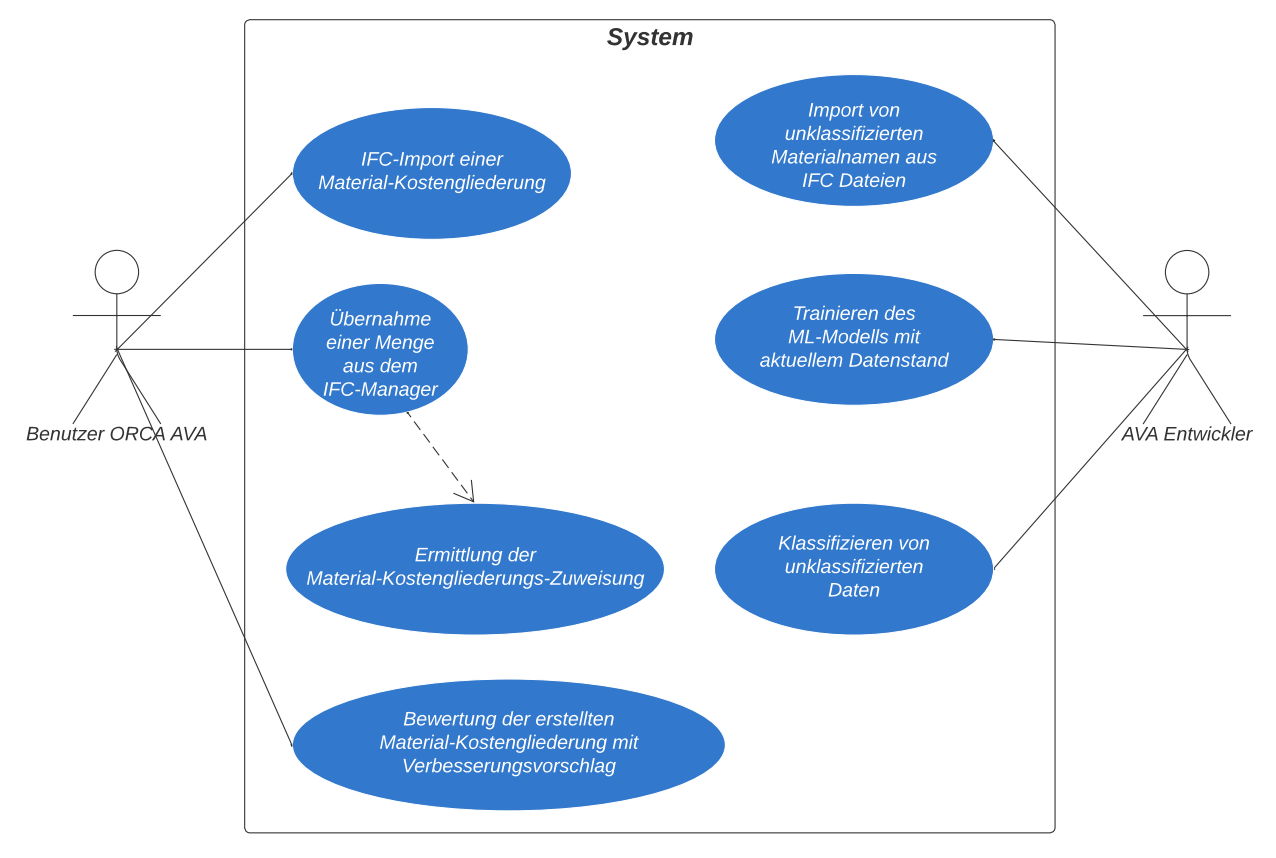
\includegraphics[width=\textwidth]{anwendungsfalldiagramm}
	\caption[Anwendungsfalldiagramm]{Anwendungsfalldiagramm}
	\label{fig:usecasediagramm}
\end{figure}

Das Ergebnis des Hauptanwendungsfalles der Material-Strukturierung ist abhängig von den Inhalten der \ac{ifc}-Datei. Durch die Nutzung verschiedener \ac{cad}-Programme und eigene Vorlieben bei der Materialangabe der ORCA AVA Benutzer entstehen viele unterschiedliche Inhalte bei der Materialangabe.
Um die hierarchische Strukturierung zu vereinfachen, werden Materialien zuerst nach dem \glqq Teile-und-hersche\grqq{} Verfahren in Oberkategorien klassifiziert. In Abbildung \ref{fig:material-categories} sind die Kategorien mit Beispielen aufgelistet. So müssen anschließend nur noch eine kleinere Liste von Materialien einer Oberkategorie weiter hierarchisch strukturiert werden.

In Abbildung \ref{fig:distribution-diagramm} ist ein Verteilungsdiagramm mit allen relevanten Objekten zu sehen. Auf dem Lokalem Computer des Benutzers laufen die beiden Prozesse der ORCA AVA und des \ac{ifc} Managers. Die ORCA AVA kommuniziert mit einem Webserver über \ac{rest}. Dieser verwaltet die anhängende SQL-Datenbank und übernimmt das Strukturieren des Material-Kostengliederungs-Import.

\subsection{Implementierung als Web-Service}
\label{c:conception:architecture:service}
Für die Materialstrukturierung ist ein neuer Webservice vorgesehen, mit den die ORCA AVA kommunizieren kann. Dies bietet einige Vorteile:

\begin{itemize}
	\setlength\itemsep{0.3em}
	\item Der Import greift immer auf das aktuellste \ac{ki}-Modell zu, welches zentral verwaltet werden kann
	\item Wegen der nötigen Verwendung von Python muss nicht bei jedem Client eine lauffähige Pythonumgebung vorhanden sein oder durchs Setup installiert werden.
	\item Neue Materialbezeichnungen und Klassifizierungen werden direkt zentral in der Datenbank persistiert.
	\item Eine Änderung/Verbesserung der Datengrundlage kann durch automatisches Trainieren direkt zu einem verbessertem \ac{ki}-Modell führen.
\end{itemize}

Für die ORCA AVA bestehen schon Services für die Bereitstellung von News, die Lizenzierung oder das Updaten der Software. Durch die Vorgabe der ORCA Software GmbH wird der Service mit dem Framework ASP.NET implementiert. ASP.NET ist ein Open-Source und Plattform-unabhängiges Web-Framework für die Entwicklung cloudbasierter Anwendungen wie Web-Applikationen, \ac{iot}-Apps oder mobile Backends. \citep{asp-net}. Die Architektur dieses Services entspricht dementsprechend den schon existierenden Services.

Daten werden über den Service in einem SQL-Datenbank Server gespeichert. Hier werden auch die ORCA Software GmbH internen Standards verwendet. Daten für den Material-Kostengliederungs-Import sind in der Tabelle \textit{Materials} persistiert. Die Tabellendokumentation ist in Abbildung \ref{fig:db-scheme} zu sehen. Zusätzlich bestehen Tabellen für die Autorisierung der Zugriffe auf den Service.

\begin{figure}[h]
	\centering
	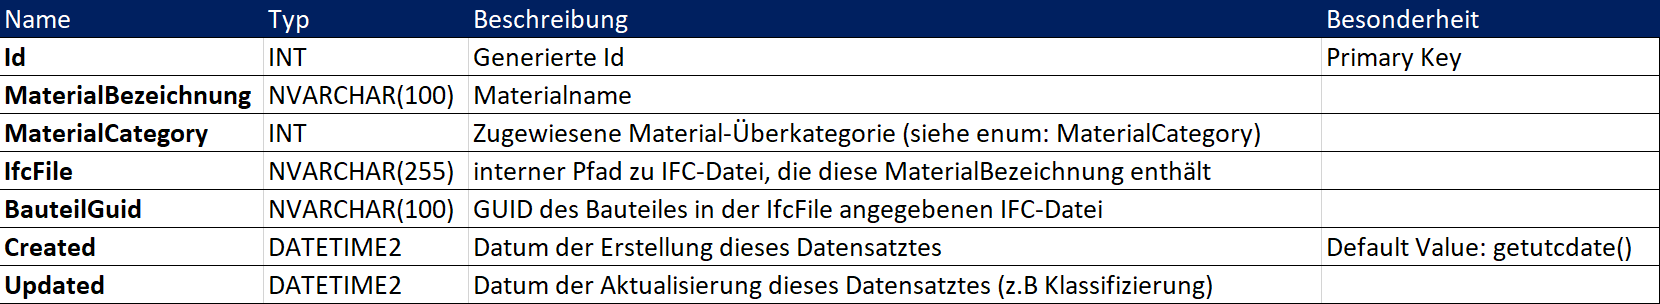
\includegraphics[width=\textwidth]{db-scheme}
	\caption[Dokumentation]{Dokumentation der Tabelle \textit{Materials} der Datenbank}
	\label{fig:db-scheme}
\end{figure}

\subsection{Konzept der Materialstrukturierung}
\label{c:conception:architecture:structuring}
Der Ablauf der Materialstrukturierung ist in drei Schritten aufgeteilt. Materialien werden nach dem Einlesen zuerst nach dem Preprocessing in Übergeordnete Kategorien klassifiziert. Danach wird jede Überkategorie nochmals feiner strukturiert.
Dieser Ablauf ist in Abbildung \ref{fig:structurize-process} anhand eines Beispiels zu sehen. Am Ende entsteht bei erfolgreicher Feinstrukturierung eine Baumstruktur mit einer Tiefe von drei. Falls in nach der Zuweisung in die Überkategorien nicht mehr als 3 Materialien in der gleichen Kategorie sind, wird nicht weiter fein-strukturiert.

\begin{figure}[h]
	\centering
	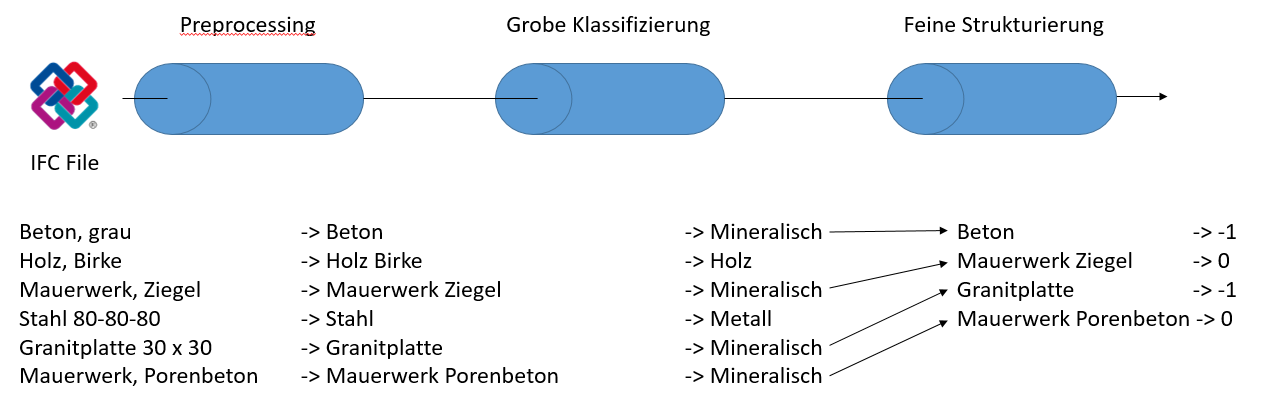
\includegraphics[width=\textwidth]{structurize-process}
	\caption[Ablauf]{Ablauf der Strukturierung mit Beispiel }
	\label{fig:structurize-process}
\end{figure}

Bei der Strukturierung von Materialien gibt es einige Probleme, die gelöst werden müssen. 
\begin{problem}
	\label{p:shorttext}
	Bei den Materialangaben handelt es sich um Sehr kurze Stichpunkte aus nur einem oder wenigen Wörtern. (z.B Metall, Edelstahl - gebürstet)
\end{problem}

Problemstellung \ref{p:shorttext} ist ein bekanntes aber noch wenig erforschtes Problem in der Textklassifizierung. Textklassifizierungen stützen sich meistens auf Textrepräsentationen. Diese machen den Text für den Klassifizierungs-Algorithmus erst lesbar. Bei der Repräsentation von Text haben kurze Texte folgende Nachteile:

\begin{itemize}
	\setlength\itemsep{0.1em}
	\item Kurzen Texten fehlt es an Kontext. Kontextbezogene Word Embeddings wie z.B. Word2Vec führen folgendermaßen zu unbrauchbaren Textrepräsentationen für die Textklassifizierung.
	\item Kurze Texte entsprechen nicht immer der Syntax der natürlichen Sprache
	\item Kurze Texte sind in der Regel mehrdeutig, weil sie
	Polyseme und Tippfehler enthalten. \citep{ijcai2017p406}
\end{itemize}

Um das Problem zu überwinden, schlagen \cite{ijcai2017p406} und \cite{chen2019deep} vor, mehr Syntax und Semantik aus den kurzen Texten zu erfassen, in dem man mit Hilfe einer bekannten Wissensbasis mit Merkmalen anreichert. Die Informationen aus dem Text alleine, reichen nicht aus um die Bedeutung des Textes in einer Textrepräsentation gut darzustellen.
\cite{Qingyuan2019} nutzt unter anderem Wikipedia2Vec, um eine Textrepräsentation der Kurztexte zu bekommen. Durch den mitgegeben Kontext über das Wikipedia2Vec Modell wird so dem Wort seine Bedeutung der Textklassifizierung mitgegeben.

\begin{problem}
	\label{p:technical-term}
	In den Materialangaben kommen viele Fachbegriffe aus der Baubranche vor.
\end{problem}
Ein weiters Problem ist Problemstellung \ref{p:technical-term}.Laut \cite{nooralahzadeh2018evaluation} gibt es viele vortrainierte Embedding Modelle, die sich aber auf den allgemeinen Bereich der Sprache fokussieren. Diese können Fachbegriffe oft schlecht verarbeiten, da die zum Trainieren genutzten Texte, diese Wörter nicht beinhalten.

Wie diese Probleme gelöst beziehungsweise umgangen werden, wird in den jeweiligen Abschnitten der verschiedenen analysierten Algorithmen in Kapitel \ref{c:conception:classification} und \ref{c:conception:fine-structuring} erläutert.

\subsection{Konzept für das Auslesen von Materialien aus einer \ac{ifc} Datei}
\label{c:conception:architecture:ifc-material-extraction}
Bevor jegliche Klassifizierung und Strukturierung stattfinden kann müssen die Materialien erst aus der \ac{ifc}-Datei extrahiert werden. In Abschnitt \ref{c:basics:ifc:buildingmaterial} wurden bereits die theoretischen Möglichkeiten der Materialangabe in der \ac{ifc}-Spezifikation aufgezählt.

Über schon vorhandenen Abstraktion des \textit{xbim-toolkit} (siehe Abschnitt \ref{c:basics:ifc:usage}) kann eine \ac{ifc}-Datei eingelesen werden. Über das instanziierte Objekt \code{IfcProject} kann dann auf alle Daten der Datei zugegriffen werden. Hier wird ein neuer \code{MaterialsManager} als Attribut des \code{IfcProject} implementiert. Über die Methode \code{Enumerable<Material> GetMergedMaterials()} im \code{MaterialsManager} können alle Materialangaben aus einer \ac{ifc}-Datei ausgelesen werden. Die Methode iteriert über jeden bekannten Materiallink mit seinem jeweiligen Objekt, teilt diese Links nach ihrem jeweiligen Materialtyp (z.b LayerSet) auf und liest die Materialbezeichnungen entsprechend dem Materialtypen aus. Am Ende liefert die Methode also alle Materialbezeichnungen in einer List mit der jeweiligen \ac{guid} des Bauteiles.
Das extrahieren der Materialien passiert Clientseitig in der ORCA AVA. So muss dem Service nicht eine ganze Datei, sondern lediglich die Liste der Materialstrings übergeben werden. Zusätzlich spart man sich die Zeit des Einlesen der Datei, wenn diese schon im \ac{ifc}-Manager geöffnet ist.

\subsection{Preprocessing der Materialien}
\label{c:conception:architecture:preprocessing}
Nach dem Einlesen beginnt das Preprocessing der Materialien.
Das Preprocessing ist ein wichtiger Schritt vor einer Klassifizierung. Es hat Auswirkungen auf die Genauigkeit, Interpretierbarkeit und Robustheit des Gesamtalgorithmus aus. \citep{Zelaya_2019} Materialbezeichnungen aus \ac{ifc}-Dateien können verrauscht und uneinheitlich sein, da es sich um ein Freitextfeld handelt. Die Vorverarbeitung der Daten hilft, die Daten zu säubern und auf das wesentliche reduzieren. \citep{Priyanga_2016}
Die Vorverarbeitungsstufe besteht normalerweise aus Aufgaben wie Tokenisierung, Entfernung von Stoppwörtern, Umwandlung in Kleinbuchstaben und Stemming. \citep{Uysal_2014}
Für die Material-Strukturierung wird das Preprocessing als erster Schritt aus der Textklassifizierung extrahiert. Somit wirkt sich das Preprocessing auf beide weiteren Schritte (Grobe Textklassifizierung und Feinstrukturierung )aus. Außerdem wird das Preprocessing zusätzlich für die Zuweisung der Materialkostengliederung bei der Mengenübernahme als erster Schritt gebraucht.
Konkret wird beim Preprocessing folgende Schritte durchgeführt. Als erstes werden alle Sonderzeichen bis auf \glqq /\grqq{} entfernt. Oft befinden sich in der Bezeichnung auch Größen- und Farbangaben, welche irrelevant für die Materialbeschaffenheit sind.
Mithilfe von Regex werden Farben, RGB-Farbcodes (z.B \textit{60 - 60 - 60}) und Größenangaben (z.B \textit{400 x 300}) herausgefiltert. Anschließend wird der Text in Worttokens, jeder Token in Kleinbuchstaben umgewandelt und unnötige Leerzeichen entfernt. Aus \textit{\glqq Kunststoff - grau 80-80-80\grqq{}} wird z.B. \textit{\glqq 'kunststoff'\grqq{}} und aus \textit{\glqq Beton- C30/37 Verputzt\grqq{}} wird \textit{\glqq 'beton', 'c30/37', 'verputzt'\grqq{}}

\section{Algorithmen für die Textklassifizierung}
\label{c:conception:classification}
Die Textklassifizierung ist nach dem Preprocessing der zweite Schritt der Material-Strukturierung. Hier werden die Materialien den in Abbildung \ref{fig:material-categories} aufgelisteten Überkategorien zugeordnet. Zuerst wird der Ablauf einer normalen Textklassifizierung erläutert und dann die Algorithmen Sdca Maximum Entropy mit ML.NET und Convolutional Neural Network mit Keras analysiert.

\subsection{Ablauf einer Textklassifizierung}
\label{c:conception:classification:steps}
Das Klassifizieren von Texten teilt sich oft in die folgende Stufen. Alle diese Stufen wirken sich auf das Ergebnis der Klassifizierung aus:

\begin{figure}[h]
	\centering
	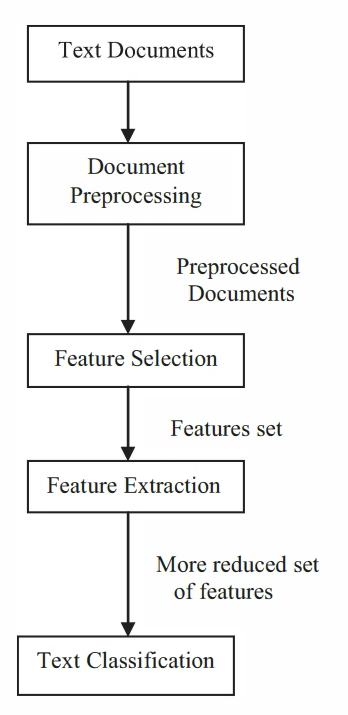
\includegraphics[width=0.3\textwidth]{classification-flow}
	\caption[Textklassifizierung]{Stufen der Textklassifizierung (Quelle:  \cite{Foram_2016})}
	\label{fig:classification flow}
\end{figure}

\paragraphheader{Preprocessing}
Das in Abschnitt \ref{c:conception:architecture:preprocessing} beschriebene Preprocessing findet als erster Schritt der ganzen Materialstrukturierung statt. Ein zusätzliches Preprocessing für die Textklassifizierung gibt es nicht.

\paragraphheader{Feature Selection}
Beim Schritt der Feature Selection werden unrelevante Informationen für die Klassifizierung aus den Ausgangsdaten entfernt. Da es bei der Materialstrukturierung nur die Materialbezeichnung als Feature gibt, muss keine Auswahl aus einem Feature-Set getroffen werden. Es werden lediglich Größen- und Farbangaben aus dem Material-String im Preprocessing entfernt.

\paragraphheader{Feature Extraction}
\begin{definition}[Feature extraction]
	\label{d:feature-extraction}
	\glqq Feature extraction addresses the problem of finding the most compact and informative set of features, to improve the efficiency or data storage and processing.\grqq{} \citep{Guyon2006}
\end{definition}
Bei der Feature Extraction geht es darum, die rohen Daten in eine numerische Darstellung zu bringen, die möglichst kompakt ist, ohne aber relevanten Informationen zu verlieren.
Auch die im Preprocessing entstandenen Worttokens sind noch Zeichenketten die in eine numerische Darstellung umgewandelt werden müssen.

\paragraphheader{Classification stages}
Nachdem die vorherigen Schritte auf die Daten ausgeführt wurde, kann die Klassifizierung starten.

\subsection{Kriterien der Messbarkeit}
\label{c:conception:classification:criteria}
Bei der Textklassifizierung ist vor allem die Genauigkeit entscheidend.


\subsection{Sdca Maximum Entropy}
\label{c:conception:classification:sdca}

\subsection{Convolutional Neural Network}
\label{c:conception:classification:cnn}


\section{Möglichkeiten für die Feinstrukturierung}
\label{c:conception:fine-structuring}
Die Feinstrukturierung ist nach der Textklassifikation der dritte Schritt der Material-Strukturierung. Hier werden die in eine Überkategorie zugeordneten Materialien weiter hierarchisch strukturiert, um eine feinere und tiefere Baumstruktur zu erreichen. In diesem Kapitel wird das Vorgehen mit dem \ac{gpt}-Modell von OpenAI und der Implementierung mit \textit{fastText} Encoding und Density Based Clustering analysiert.

\subsection{Spezifikation und Kriterien der Messbarkeit}
\label{c:conception:fine-structuring:criteria}
Die Verteilung der Materialien auf die Überkategorien ist nicht gleich verteilt. Materialien der Kategorien \textit{Mineralisch} oder \textit{Metall} kommen kommen viel häufiger vor als zum Beispiel \textit{BitumenUndTeer} oder \textit{Gebäudetechnik}. Nicht in jeder \ac{ifc}-Datei ist eine Einfahrt aus Asphalt oder die Gebäudetechnik definiert. Die Verteilung der Materialien ist in Tabelle \ref{t:distribution} zu sehen. Somit ist auch die Verteilung der Materialien aus einer \ac{ifc}-Datei nach dem Schritt der Textklassifizierung in die Überkategorien nicht gleich verteilt. Eine Feinstrukturierung ist bei zwei Materialien pro Kategorie nicht sinnvoll und auch bei drei soll noch keine tiefere Strukturierung stattfinden. Erst bei vier Materialien pro Kategorie wird feiner strukturiert.
Die Feinstrukturierung soll keine weiteren selbst trainierten Klassifizierungsmodelle benötigen. Diese würden zusätzlich zu der Textklassifizierung hohen Wartungsaufwand verursachen, da sie regelmäßig aktualisiert werden müssten, um die Genauigkeit der Klassifizierung beizubehalten bzw. zu verbessern. In den folgenden Kapiteln wird dies einerseits mit dem Benutzen eines fertig trainierten Modells und Unsupervised Learning umgangen.
Somit kann die Feinstrukturierung nicht mit fest definierten Kriterien der Algorithmen evaluiert werden. Für die Auswertung sind 20 Beispiele zum Testen der Algorithmen definiert. Diese sind in Anhang \ref{c:tables} von Tabelle \ref{t:evaluation-example1} bis \ref{t:evaluation-example22} zu finden. Die Beispiele wurden in Kooperation mit dem Produktmanagement erstellt und fachlich überprüft. Sie sind auf Basis echter \ac{ifc}-Dateien entstanden. Eine Tabelle stellt alle Materialien einer \ac{ifc}-Datei, die in die Überkategorie (in der Überschrift zu sehen) eingeordnet wurden, dar. In der Spalte \textit{Klasse} sind die Begriffe einer Unterklasse über eine Nummer zugeordnet. Alle Begriffe mit der selben Nummer gehören zu einer Unterklasse. Die Verteilung der Beispiele über die Überkategorien ist aus dem selben Grund, wie auch die Verteilung der Materialklassifikationsdaten (Tabelle \ref{t:distribution}), nicht gleich verteilt. Die Ergebnisse der Evaluation sind in Abschnitt \ref{c:comparison:fine-structuring} aufgezeigt.

% Tabelle
\begin{table}[h]
	\centering
	\begin{tabular}{|l|l|l|}
		\hline
		\textbf{Kategorie} & \textbf{Anteil} & \textbf{Anzahl} \\ \hline
		Metall  & 25\% & 119 \\ \hline
		Glas & 4\% & 17 \\ \hline
		Holz & 9\% & 43 \\ \hline
		Kunststoff & 8\% & 39 \\ \hline
		BitumenUndTeer & 1\% & 3 \\ \hline
		Mineralisch & 26\% & 127 \\ \hline
		Verbundbauteile & 5\% & 22 \\ \hline
		Dämmungen & 8\% & 39 \\ \hline
		GebäudeTechnik & 1\% & 6 \\ \hline
		Sonstiges & 14\% & 70 \\ \hline
		\textbf{Gesamt} & 100\% & 485 \\ \hline
	\end{tabular}
	\caption{Verteilung der Materialklassifikationsdaten}
	\label{t:distribution}
\end{table}

\subsection{\acf{gpt} Modell von OpenAI}
\label{c:conception:fine-structuring:openai}
OpenAI ist ein Unternehmen für \ac{ki}-Forschung und -Einsatz. Sie bieten verschiedene fertig trainierte \ac{ki}-Modelle über eine \ac{api} an. Neben Speech-ToText und einem Bildgenerierungsmodell gibt es das Sprachverarbeitungsmodell \ac{gpt}.
Die Nutzung eines fertig trainierten Modells hat einige Vorteile. Vor allem werden so die Problemstellungen \ref{p:shorttext} und \ref{p:technical-term} automatisch gelöst. OpenAI benutzen ihr eigenen ausgereiften Textrepräsentationsmodelle. Somit wird auch die Bedeutung von Worten bei den kurzen Materialangaben bei der Vektorisierung beibehalten. Außerdem kann das Modell durch die Masse an Trainingsdaten aus Büchern, Artikel und Webseiten auch mit vielen Fachbegriffen umgehen. Außerdem spart man sich die Wartung eines selbst trainierten Modells. Das Etikettieren von Daten ist sehr Zeit und auch Ressourcen-aufwändig, da es von einer Person gemacht werden muss, die passende fachliche Kenntnisse besitzt.

Der Begriff \ac{gpt} steht für eine Reihe von vor trainierten Sprachmodellen, die von OpenAI entwickelt wurden. Diese sind populäre Transformer für die Generierung von natürlicher Sprache. \citep{zhu_luo_2022}
\begin{definition}[Transformer]
	\glqq Transformers are a type of artificial neural network architecture that is used to solve the problem of transduction or transformation of input sequences into output sequences in deep learning applications. \grqq{} \citep{Rogel-Salazar2022-pd}
\end{definition}
\ac{gpt} ist also ein Modell, das auf einem großen Datensatz an textuellen Informationen trainiert wurde und kann zur Bewältigung spezifischer sprachbezogener Aufgaben eingesetzt werden. Im Vergleich zu Modellen zum Verstehen natürlicher Sprache wie zum Beispiel BERT kann \ac{gpt} natürliche Sprache generieren. Der Algorithmus liefert basierend auf allen eingegebenen Tokens neue Tokens, welche dann die Antwort darstellen. \citep{zhu_luo_2022}

OpenAI hat verschiedene Versionen des \ac{gpt} Algorithmus. \ac{gpt} 1 wurde 2018 veröffentlicht. Darauf folgte \ac{gpt} 2 2019. Beide Modelle wurden in zwei Schritten trainiert. Zuerst wurde ein Model mit Hilfe von Unsupervised Learning mit einer sehr großen Datenmenge vor trainiert und konnte dann für bestimmte Aufgaben mit dem Trainieren von überwachten Datensätzen verfeinert werden. \citep{alec_2018} \ac{gpt} 3 wurde in einem Schritt trainiert und verzichtet auf die kontextbezogene Verfeinern des Modells. \citep{zhu_luo_2022} Stattdessen benutzt das Modell \glqq Meta-Learning\grqq{}. Das Modell entwickelt so beim Training ein breites Spektrum an Mustererkennungsfähigkeiten und weiteren Fertigkeiten, die sich beim Ausführen des Modells schnell an die gewünschte Aufgabe anpassen. 
Durch die Skalierung des Modells auf 175 Billionen Parameter wurden ähnliche Ergebnisse wie bei damaligen modernster fein abgestimmter Systeme erzielt. \citep{brown2020language} 

Die \ac{gpt}-Modelle 2 und 3 sind nicht darauf trainiert, Benutzeranweisungen zu befolgen. Dafür wurde 2022 \textit{InstructGPT} auf der Basis des \ac{gpt} 3 Modell trainiert. Mit Supervised Learning und Reinfocement Learning wurde das Modell verfeinert, um hilfreichere Ergebnisse bei Benutzeranweisungen zu bekommen. Zusätzlich wurde eine Reduktion von toxischen Antworten erzielt. \citep{ouyang2022training}

Das für die Material-Feinstrukturierung verwendete Modell \textit{ChatGPT} ist ein Zwillingsmodell von \textit{InstructGPT} und ist ist eine Feinabstimmung eines Modells der \ac{gpt}-3.5-Serie. \citep{OpenAI2022-la}
Das Modell wurde Ende 2022 veröffentlicht und ist über eine öffentliche API erreichbar und kann mit Hilfe des Python-Package \textit{openai} leicht genutzt werden.

\subsection{fastText mit \acf{dbscan}}
\label{c:conception:fine-structuring:dbscan}
In diesem Ansatz werden mit Hilfe von Clustering, Materialien weiter strukturiert. Durch das Nutzen von Unsupervised Learning müssen so keine weiteren Klassifizierungs-Modelle trainiert und verwaltet werden.
Um Problemstellung \ref{p:shorttext} zu lösen, wird das Vorgehen wie es auch \cite{Qingyuan2019} vorgeschlagen hat angewandt. Ein Textrepräsentationsmodell wird mit anderen Texten trainiert und mit diesem Modell die Vektorisierung auf die Materialbezeichnungen angewandt. 
Die \glqq ORCA Software GmbH\grqq{} entwickelt neben der ORCA AVA das Portal \ac{ade}. Dieses hat über einer Millionen Ausschreibungstext von über 800 verschiedenen Herstellern. Diese Texte eignen sich optimal für das Trainieren des Worteinbettung Modells. Sie enthalten viele Materialnamen und weitere Fachbegriffe der Baubranche, welche essenziell für das Clustering der Materialien aus dern \ac{ifc}-Dateien sind. Somit ist zusätzlich Problemstellung \ref{p:technical-term} gelöst. Auch \cite{nooralahzadeh2018evaluation} kommt auf das Ergebnis, dass sich Domänen-Spezifische Word Embeddings auch schon mit limitierter Eingabedaten nützlich ist. 
Die Ausschreibungstexte werden mit einem schon existierendem Preprocessing verarbeitet und liefern am Ende ca. 360.000 Sätze mit über 300.000 verschiedene Wörtern. Im Preprocessing werden verschiedene Zeichenketten aus den Texten mit Hilfe von Regex herausgefiltert. Dazu gehören \ac{url}s, verschieden Normen wie \ac{din} und Attribut-Listen wie zum Beispiel \textit{Nettogewicht: 0,196 kg}. Zusätzlich werden unnötige Absätze entfernt.
Auch wenn Ausschreibungstexte oft keine kompletten Sätze beinhalten, werden so viele nicht relevanten Daten entfernt.

Als Textrepräsentation und Wort-Einbettungs-Algorithmus bietet sich \textit{fastText} an. \textit{fastText} wurde 2016 von Facebook veröffentlicht \citep{fastText_release2016}. Außerdem wurde die dazu getätigte Forschung mit \cite{bojanowski2017enriching} und \cite{joulin2016bag} veröffentlicht.

Das Modell basiert auf dem Wort-Einbettungs Algorithmus \textit{Word2Vec} mit \glqq Continuous Skip-Gram\grqq{} und \ac{cbow} \citep{bojanowski2017enriching}. Das Modell nutzt ein Neuronales Netz bei dem die ausgewählten Gewichte als Vektor für ein Wort entstehen. Die Trainingsdaten für das neuronale Netz entstehen durch ein selbst gestelltes Problem. Mit \ac{cbow} versucht man mit nahegelegenen Wörtern ein Wort hervorzusagen. Bei Skip-Gram versucht man aus einem Wort den Kontext, also die nahegelgenden Wörter hervorzusagen. So kann beim Iterieren über den Trainingstext das Modell immer weiter trainiert werden. In Abbildung \ref{fig:cbow} sieht man ein \ac{cbow} Beispiel, in dem die Kontextwörter als Input Layer und das gesuchte Wort als Ergebnis zur Ermittlung des Verlustes genutzt werden. Die nach dem Trainieren entstandenen Gewichte \textit{W1\textsubscript{n$\times $k}}\: sind dann die Repräsentation für das Wort \textit{catches}.
\begin{figure}[h]
	\centering
	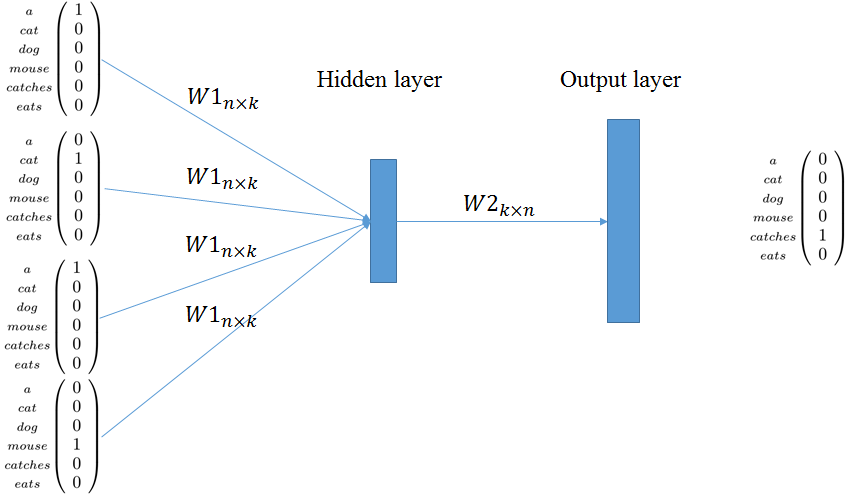
\includegraphics[width=\textwidth]{cbow-model}
	\caption[CBOW]{Beispiel des \ac{cbow}-Modells. (Quelle:  \cite{cbow_image})}
	\label{fig:cbow}
\end{figure}
\textit{fastText} erweitert diese Vorgehensweise und, nutzt \textit{fastText} Teilwortinformationen und ein Wort als Vektor darzustellen. Wörter werden in N-Grams dargestellt. \citep{bojanowski2017enriching} Die Repräsentation für das Wort \textit{Estrich} mit n = 3 ist zum Beispiel \textit{<Es,est,str,tri,ric,ich,ch>} wobei die Zeichen \textit{<} und \textit{>} als Begrenzungszeichen hinzugefügt werden, um die N-Gramms eines Wortes vom Wort selbst zu unterscheiden. Wäre also das Wort \textit{ich} im Vokabular, wird es als \textit{<ich>} dargestellt. Das Neuronale Netz wird dann mit der Liste der N-Gramms inklusive dem kompletten Wort trainiert. Somit ermöglicht das Modell die gemeinsame Nutzung der Teilwortinformationen für alle Wörter\citep{bojanowski2017enriching}. Zusätzlich nutzt \textit{fastText} eine hierarchische Softmax Verlustfunktion, um die Berechnung von unausgewogenen Verteilungen zu beschleunigen \citep{fastText_release2016}.

\textit{fastText} hat für den Anwendungsfall folgende Vorteile:

\begin{itemize}
	\item \textit{fastText} kann mit Wörtern außerhalb des Vokabulars umgehen. Bei unbekannten Wörtern, werden die Vektoren der einzelnen Char-Ngramms summiert. Es muss allerdings mindestens eines der char-ngrams in den Trainingsdaten vorhanden sein. \citep{gensim_fastText,le2014distributed} Da sich bei diesem Konzept der Feinstrukturierung das Vokabular bei Ausführung vom Trainingsvokabular unterscheidet, ist das Verarbeiten von diesen Wörtern essentiell.
	\item \textit{fastText} liefert Vektordarstellungen mit fester Länge welche für das Clustering mit zum Beispiel \ac{dbscan} nötig ist. \citep{le2014distributed}
	\item \textit{fastText} liefert bessere Ergebnisse bei syntaktischen Aufgaben als zum Beispiel \textit{Word2Vec} und \textit{Bag of Words} \citep{fastText_word2vec_comparison,le2014distributed}
	\item \textit{fastText} hat eine schnellere Trainingszeit als vergleichbar genaue Deep Learning Algorithmen \citep{fastText_release2016}
\end{itemize}


Mit dem fertige trainierten \textit{fastText} Modell können dann Wörter in Vektoren umgewandelt werden. Bei der Vektorisierung der Materialien, die aus mehreren Wörtern bestehen, werden die Vektoren der einzelnen Wörter aufaddiert. Das ist die selbe Vorgehensweise, wie \textit{fastText} bei neuen Wörter, die nicht im Vokabular vorkommen, vorgeht \citep{gensim_fastText}.


Wenn die Materialbezeichnungen vektorisiert wurden können sie geclusterd werden. Aus einer großen Auswahl an Cluster-Algorithmen bietet sich \ac{dbscan} an. \glqq The \ac{dbscan} algorithm views clusters as areas of high density separated by areas of low density.\grqq{} \citep{scikitlearn_clustering} Der Algorithmus wurde \citeyear{Ester1996ADA} von \citeauthor{Ester1996ADA} vorgestellt und veröffentlicht. Ziel war es einen Algorithmus zu entwickeln, bei dem man wenig Fachwissen für die Bestimmung der Parameter braucht, Cluster mit beliebiger Form bekommen kann und eine gute Effizienz bei großen Datenbanken besitzt.

\ac{dbscan} braucht die zwei Parameter \textit{min\_samples} und \textit{eps}. Als erster Schritt werden alle Punkte, die inklusive sich selbst mindestens \textit{min\_samples} an Nachbarn innerhalb des Abstands von \textit{eps} hat, als Kernpunkte definiert. Alle anderen Punkte werden erstmals als Rauschen gekennzeichnet. Als nächstes werden alle Kernpunke, die inherhalb des Radius \textit{eps} beieinander liegen als ein Cluster definiert. Zum Schluss werden nochmal alle Rauschpunke überprüft, ob sie nicht doch innerhalb des Radius eines Kernpunktes in einem Clusters liegen. \citep{scikitlearn_clustering,Ester1996ADA} Die Anzahl der Cluster ist also abhängig von den Daten (und den Parametern) und muss nicht vorgegeben werden.
\ac{dbscan} hat also für den Anwendungsfall folgende Vorteile:

\begin{itemize}
	\item \ac{dbscan} liefert eine passende Anzahl von Clustern, abhängig von den Materialbezeichnungen. Dies ist wichtig, da die Anzahl der Materialien pro Überkategorie und somit auch die der potentiellen Clustern immer unterschiedlich ist. Das Ergebnis des Clustering wird auch direkt dem Benutzer der ORCA AVA präsentiert. Somit ist es auch nicht möglich mit einem anderen Clustering-Algorithmus über die Anzahl von Clustern zu iterieren und das fachlich beste auszuwählen.
	\item Es müssen keine Trainingsdatensätze oder Modell verwaltet werden.
	\item Der Algorithmus setzt die mitgegebene Bedeutung des Wortes bei der Wort-Einbettung mit \textit{fastText} um. 
\end{itemize}

Am Ende liefert \ac{dbscan} zu jedem übergebenem Material eine Zahl, die das Cluster repräsentiert. Rauschpunkte werden mit -1 zurückgegeben. Diese werden dann nicht weiter strukturiert und bleiben hierarchisch direkt unter ihrer zugewiesenen Überkategorie. Dieses Format kann für die Evaluationsbeispiele (Tabelle \ref{t:evaluation-example1} - \ref{t:evaluation-example22}) direkt genutzt werden. Bei diesem Ergebnis fehlen für die endgültige Material-Strukturierung noch die Begriffe der Gliederungspunkte für die entstandenen Cluster.

\chapter{Gegenüberstellung der möglichen Konzepte}
\label{c:comparison}
In diesem Kapitel werden die in Kapitel \ref{c:conception} vorgestellten Konzepte verglichen.
Dies wird gesondert für die Textklassifizierung und die Feinstrukturierung durchgeführt. Es wird jeweils das Ergebnis ausgewertet und eine Auswahl eines Algorithmus durchgeführt.
\section{Vergleich der Textklassifizierung}
\label{c:comparison:classification}
\subsection{Auswertung}
\label{c:comparison:classification:evaluation}
\subsection{Auswahl eines Algorithmus}
\label{c:comparison:classification:selection}
\section{Vergleich der Feinstrukturierung}
\label{c:comparison:fine-structuring}
\subsection{Auswertung}
\label{c:comparison:fine-structuring:evaluation}
\subsection{Auswahl eines Algorithmus}
\label{c:comparison:fine-structuring:selection}


\chapter{Praktische Umsetzung}
\label{c:implementation}
In diesem Kapitel wird die Umsetzung der ausgewählten Algorithmen und Bibliotheken beschrieben. Zuerst werden Die Implementierung des Services und der Python-Interop gezeigt. Danach geht es um die konkrete Implementierung der Material-Strukturierung.

\section{Implementierung des ASP.NET Services}
\label{c:implementation:service}
Die Realisierung als ASP.NET Service ist eine Anforderung der \glqq ORCA Software GmbH\grqq{}. Für das Erstellen eines neuen Services gibt es ein fertiges Projekttemplate, weleches nur umbenannt werden muss. Die Vorlage liefert eine einheitliche Projektstruktur und zeigt den Aufbau des Services anhand der Implementierung eines Beispiels. Die neu genannte \textit{ MaterialStructurizationApi} hat zwei verschiedene \ac{rest}-Controller.
Diese teilen sich wie im Anwendungsfalldiagramm (Abbildung \ref{fig:usecasediagramm}) zu sehen in die Schnittstellen für die ORCA AVA Benutzer und die ORCA Internen Schnittstellen auf. In den Controllern werden die \ac{rest}-Schnittstellen-Methoden definiert. Dazu zählt die Art der Anfragemethoden, die \ac{url} oder auch die möglichen Antwort-StatusCodes. Service interne Logik wird im \code{MaterialService} organisiert. Hier werden die \acp{dto} in Entitäten umgewandelt und die Aufrufe auf die entsprechenden weiteren themenspezifischen Services oder Datenzugriff-Repositories weitergeleitet. Am Ende werden Rückgabewerte wieder in entsprechende \acp{dto} abgebildet und an den Controller zurückgegeben. Ein Beispiel ist in Abbildung \ref{lst:materialservice} zu sehen. Die Methode ist für die Material-Strukturierung zuständig. Sie bekommt die Liste von Manualbezeichnungen und eine \code{bool}, welcher bestimmt ob die Feingliederung durchgeführt werden soll, übergeben. Nach der Parameterprüfung werden Duplikate aus der Materialliste entfernt und danach in Zeile 8 über das \code{MaterialRepository} neue Materialien dem Trainingsdatensatz für die Klassifizierung hinzugefügt. Danach wird der \code{MaterialStructurizerService} aufgerufen, der sich dann um die Logik der Strukturierung kümmert.

Repositories kapseln den Datenzugriff über Interfaces. So ist die Logikimplementierung in den Services unabhängig von der Implementierung des Datenbankzugriffs. Der Datenbankzugriff wird in den Repositories mit der Object-Relation-Mapper Bibliothek \textit{EntityFramework} implementiert. Es wird der Model-First Ansatz verwendet, bei dem zuerst die Objektstruktur im C\#-Code definiert wird und daraus automatisiert die Datenbank generiert wird.

\section{Python-Interop}
\label{c:implementation:python-interop}
Für die Implementierung einiger Komponenten wird Python als Programmiersprache benötigt. Der Webservice wird allerdings mit ASP.NET implementiert. Um die Kommunikation zwischen .NET und Python zu vereinfachen wird das Nuget-Packet \code{pythonnet} verwendet. Die Bibliothek vereinfacht es Python-Code aus dem C\#-Code auszuführen und verschiedene Python-Variablen auszulesen oder diesen Werte zuweisen. Um den Python-Interop nutzen zu können, muss eine lauffähige Python-Umgebung installiert sein. Der Python-Interop ist in mit dem Interface \code{IKiExecuter} gekapselt und lässt so eine eventuelle C\# Ablösung der Python-Komponenten in der Zukunft einfach zu integrieren. In Listing \ref{lst:pythonnet} ist der Python-Code Aufruf für das Preprocessing zu sehen. Nachdem die Python-Engine initialisiert wird, kann der Python-Variable ein Wert zugewiesen werden. Dann wird das Skript \textit{preprocess.py} (Listing \ref{lst:preprocess}) über den Namen aufgerufen und danach die Python-Variable \code{material\_preprocessed}, in welcher am Ende des Python-Skripts das Ergebnis steht, wieder ausgelesen.

\lstinputlisting[language={[Sharp]C}, caption={Python-Interopt für das Preprocessing}, style={csharp}, label={lst:pythonnet}]{Pythonnet.cs}

Zusätzlich löst \textit{pythonnet} das Problem, dass das Pythonskript zur Feinstrukturierung nicht immer wieder das \textit{fastText}-Modell neu in den Speicher laden muss. Durch die Möglichkeit Python-Variablen zuzuweisen und auszulesen, ist es auch möglich das \textit{fastText}-Modell initial beim Starten des Services in den Speicher zu laden. Das macht das Ausführen der Feinstrukturierung sehr viel performanter und erst produktiv einsetzbar.
Für die Entwicklung der Pyhtonskripte wird die Logik immer in eine Methode ausgelagert. Mit der Zeile \code{if \_\_name\_\_ == "\_\_main\_\_":} wird der darauf folgende Code beim initialen aufrufen des Skriptes ausgeführt. Mit dem Try-Except-Block wird überprüft, ob durch \textit{pythonnet} die Eingabevariable schon initialisiert wurde. Ansonsten kann beim Debuggen ein Wert über die Kommandozeile eingetragen werden. Somit kann für alle Konstellationen immer nur ein Skript verwendet werden. Das ganze Skript sowohl die definierte Methode kann dann mit \textit{pyhtonnet} im C\#-Code ausgeführt und aber auch autark im Debug-Modus ausgeführt werden. (Beispiel: Codeausschnitt \ref{lst:preprocess})

\section{Implementieren des Auslesens aller Materialien aus einer \ac{ifc} Datei}
\label{c:implementation:ifc-material-extraction}
Für das Auslesen aller Materialien aus einer \ac{ifc}-Datei besteht schon ein Grundgerüst in der Codebasis der ORCA AVA. Es bestehen bereits die Funktionen mit dem \textit{xbim-toolkit} \ac{ifc}-Dateien einzulesen und daraus das Business Model \code{IfcProject} zu erzeugen. Dazu reicht der Pfad zur gewünschten \ac{ifc}-Datei. 

\section{Implementierung der Material-Strukturierung}
\label{c:implementation:structuring}
Die Implementierung der Material-Strukturierung teilt sich ähnlich wie in Kapitel \ref{c:conception} auf. Zuerst geht es um das Erstellen einer Datengrundlage, dann um die Implementierung des Preprocessings. Anschliesend wird das Textklassifizierungs-Modell vorgestellt. Für die Feinstrukturierung wird am Ende noch die Implementierung für \textit{fastText} und \ac{dbscan} erläutert.
\subsection{Erstellen einer Datengrundlage}
\label{c:implementation:data} 
Die Datengrundlage entstand durch das Extrahieren der Materialangaben (wie in Abschnitt \ref{c:implementation:ifc-material-extraction} beschrieben) aus verschiedenen \ac{ifc}-Dateien. Hierzu standen über 500 verschiedene Dateien zur Verfügung. Die daraus entstandenen Materialbezeichnungen wurden über eine \ac{http}-PUT Anfrage in einem \ac{sql}-Server mit dem in Abbildung \ref{fig:db-scheme} abgebildetem Schema persistiert. Die Liste diese Materialien wurden anschließend manuell gefiltert. In vielen \ac{ifc}-Dateien werden die Möglichkeiten der Materialangabe noch nicht gut genutzt. Deshalb waren viele Materialangaben nicht aussagekräftig um sie als Trainingsdaten für die Textklassifizierung zu nutzten. Am Ende standen circa 500 unterschiedliche Materialien zur Verfügung.
Um die Daten anschließend zu klassifizieren, wurde ein Klassifizierungs-Service mit Oberfläche implementiert (siehe Anhang \ref{fig:classification-service}). Dieser stand im internen Firmennetzwerk zur Verfügung, sodass ausgewählte Mitarbeiter die Materialien klassifizieren konnten. Die dafür benötigten Methoden standen über den \code{InhouseMaterialController} der \textit{MaterialStructurizationApi}, welcher die internen ORCA-Schnittstellen bietet, zur Verfügung. Somit wurden über 480 klassifizierte Datensätze geschaffen. Die Verteilung der Klassifizierung ist in Abbildung \ref{fig:distribution-diagramm} zu sehen.
\subsection{Implementierung des Preprocessings}
\label{c:implementation:preprocess}
Das Preprocessing für die Textklassifizierung wurde in Python implementiert.
Das Vorgehen wurde schon in Abschnitt \ref{c:conception:architecture:preprocessing} erläutert. Die Implementierung des Pythonskripts ist im Codeausschnitt \ref{lst:python-preprocess} zu sehen. Das Preprocessing basiert größtenteils auf der Textverarbeitung mit Regex. Mit dem Regex \code{[A-Za-z0-9üäöÜÄÖßóåéèÉÈÓ/]} werden alle Sonderzeichen bis auf  \glqq /\grqq{} aus dem String entfernt. Bei der Maßangabe mussten aufgrund der unterschiedlicher Verarbeitung des Python-Package \code{re} bei \code{re.findall(...)} \code{re.sub(...)} mehrere Regex definiert werden. Zuerst werden dreidimensionale Maße im Materialstring gesucht. Wenn keine Vorhanden sind, werden zweidimensionale Maße entfernt. Ansonsten wird mit einem zusätzlichen Regex die dreidimensionalen Maßangaben entfernt. Am Ende wird eine Liste von Strings aus dem Materialstring gefiltert und überschüssige Leerzeichen mit \code{strip()} entfernt. 

Wie in Abbildung \ref{fig:db-scheme} zu sehen ist, werden die vorverarbeiteten Materialien in der Datenbank persistiert. Immer wenn ein neues Material in die Datenbank geschrieben wird, wird das Preprocessing gestartet. Das bietet die Möglichkeit direkt nach dem Klassifizieren eines Materials, das Textklassifizierungs-Modell ohne vorheriges Preprocessing neu trainieren zu können. Dadurch verringert sich die Ausführungszeit des Trainingsprozesses und es kann direkt auf das aktualisierte Modell zugegriffen werden.
\subsection{Training des Text-Klassifizierungsmodells}
\label{c:implementation:classification-training}
\subsection{Training des \textit{fastText} Modells}
\label{c:implementation:embedding-training}
Für das Trainieren des \textit{fastText}-Modells wird die Python-Bibliothek \textit{Gensim}  \citep{rehurek_lrec} verwendet. Die Bibliothek implementiert verschiedene Vektorisierungsalgorithmen, wie zum Beispiel \textit{Word2Vec}, \textit{EnsembleLDA} aber auch \textit{fastText}.

Über eine interne Schnittstelle wurden alle \ac{ade}-Texte in Textdateien gespeichert. Der Trainingsablauf wurde in drei Skripte aufgeteilt. Das Skript \textit{fasttext\_prepare.py} liest die Catalogtexte ein und führt das in Abschnitt \ref{c:conception:fine-structuring:dbscan} erläuterte Preprocessing aus.
Das Skript \textit{fasttext\_train.py} liest die vorverarbeiteten Texte wieder ein teilt sie in Sätze ein und generiert Tokens aus jedem Satz. Bei der Aufteilung in Sätze werden Abkürzungen in denen ein Punkt vorkommt beachtet und führen zu keinem eigenen Satz. Anschließend wird ein \textit{fastText}-Modell initialisiert, trainiert und am Ende gespeichert.

Mit dem dritten Skript \textit{fasttext\_test.py} kann man das trainierte Modell fachlich bewerten. Mit der Methode \code{most\_similar(positive=[word],topn=100)} werden die 100 ähnlichsten Wörter zu einem Wort ausgegeben. Da der Algorithmus \ac{dbscan} mit der Dichte von Punkten und somit der \glqq Ähnlichkeit\grqq{} von Worten funktioniert, ist diese Methode eine gutee Möglichkeit das Modell fachlich zu evaluieren und testen.
\subsection{\ac{dbscan} Clustering}
\label{c:implementation:clustering}





\chapter{Maßnahmen zur Qualitätssicherung}
\label{c:qs}
\section{Clean Code}
\label{c:qs:cleancode}
\section{Technische Hilfsmittel}
\label{c:qs:technical_aids}
Bei der Durchsetzung von Maßnahmen der Qualitätssicherung wurden technische Hilfsmittel verwendet. Diese sind Visual Studio, Visual Studio Code, SonarQube, Azure DevOps und CI/CD. Auf diese wird in diesem Abschnitt eingegangen.
\section{Tests und Abnahme}
\label{c:qs:tests}


\chapter{Abschluss}
\label{c:closing}

\section{Bewertung der praktischen Umsetzung}
\label{c:closing:rating}
\section{Fazit}
\label{c:closing:conclusion}
\section{Integration in die ORCA AVA}
\label{c:closing:integration}
\section{Ausblick}
\label{c:closing:outlook}
Die Erweiterung soll in der Version 26 in der ORCA AVA Enterprise Edition erscheinen.

Fachlich: Nutzung der Materialliste für die CO2-Bilanz einer \ac{ifc}-Datei
